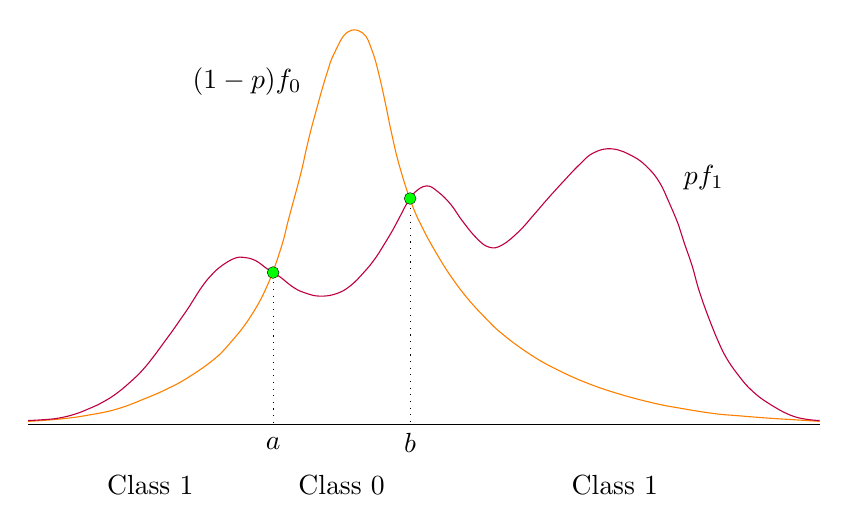
\begin{tikzpicture}
    % (1-p) f_0
    \draw [orange] plot[smooth, tension=.7] coordinates {
        (-4.88,-2.09) (-4.47,-2.06) (-4.11,-2.01) (-3.74,-1.93) (-3.37,-1.79)
        (-3.12,-1.68) (-2.86,-1.54) (-2.53,-1.31) (-2.32,-1.10) (-2.07,-0.78)
        (-1.85,-0.38) (-1.67, 0.11)  % first crossing (a)
        (-1.57, 0.49) (-1.42, 1.05) (-1.35, 1.36) (-1.29, 1.61) (-1.23, 1.83)
        (-1.15, 2.12) (-1.08, 2.35) (-1.00, 2.57) (-0.83, 2.85) (-0.63, 2.84)
        (-0.51, 2.61) (-0.42, 2.29) (-0.34, 1.93) (-0.27, 1.59)
        (-0.17, 1.17) (-0.02, 0.70)  % second crossing (b)
        ( 0.13, 0.36) ( 0.33, 0.00) ( 0.51,-0.28) ( 0.70,-0.53) ( 0.91,-0.76)
        ( 1.14,-0.98) ( 1.51,-1.25) ( 1.87,-1.45) ( 2.26,-1.62) ( 2.65,-1.75)
        ( 3.07,-1.86) ( 3.38,-1.92) ( 3.82,-1.99) ( 4.15,-2.02) ( 4.53,-2.05)
        ( 4.85,-2.07) ( 5.17,-2.09)
    };
    \node at (-2.10, 2.23) {$(1-p)f_{0}$};  % label

    % p f_1
    \draw [purple] plot[smooth, tension=.7] coordinates {
        (-4.88,-2.08) (-4.70,-2.07) (-4.50,-2.05) (-4.29,-2.00) (-4.11,-1.93)
        (-3.94,-1.85) (-3.75,-1.73) (-3.55,-1.56) (-3.42,-1.43) (-3.29,-1.27)
        (-3.15,-1.08) (-3.04,-0.93) (-2.95,-0.80) (-2.84,-0.64) (-2.68,-0.39)
        (-2.56,-0.24) (-2.43,-0.12) (-2.26,-0.02) (-2.13,-0.01) (-1.99,-0.05)
        (-1.85,-0.15) (-1.69,-0.25)  % first crossing (a)
        (-1.51,-0.39) (-1.36,-0.46) (-1.18,-0.50) (-0.97,-0.47) (-0.79,-0.37)
        (-0.61,-0.19) (-0.48,-0.03) (-0.37, 0.14) (-0.25, 0.34) (-0.18, 0.47)
        (-0.07, 0.68) ( 0.02, 0.81)  % second crossing (b)
        ( 0.18, 0.90) ( 0.33, 0.82) ( 0.49, 0.66) ( 0.63, 0.46) ( 0.82, 0.23)
        ( 0.98, 0.12) ( 1.14, 0.15) ( 1.35, 0.32) ( 1.53, 0.52) ( 1.72, 0.74)
        ( 1.92, 0.96) ( 2.12, 1.17) ( 2.30, 1.32) ( 2.54, 1.37) ( 2.81, 1.27)
        ( 3.00, 1.12) ( 3.14, 0.94) ( 3.25, 0.71) ( 3.38, 0.40) ( 3.45, 0.18)
        ( 3.55,-0.11) ( 3.64,-0.43) ( 3.76,-0.77) ( 3.89,-1.09) ( 3.99,-1.29)
        ( 4.12,-1.48) ( 4.29,-1.68) ( 4.52,-1.86) ( 4.85,-2.03) ( 5.17,-2.08)
    };
    \node at ( 3.70, 1.01) {$pf_{1}$};  % label

    % first crossing (a)
    \draw (-1.77,-0.20) node (a) {} circle (2pt);  % circle (a)
    \fill [green, thick] (a) circle (2pt);         % fill circle
    \draw [dotted] (a) -- (-1.77,-2.13);           % dotted line to x-axis
    \node at (-1.77,-2.37) {$a$};                  % label on x-axis

    % second crossing (b)
    \draw (-0.03, 0.74) node (b) {} circle (2pt);  % circle (b)
    \fill [green, thick] (b) circle (2pt);         % fill circle
    \draw [dotted] (b) -- (-0.03,-2.13);           % dotted line to x-axis
    \node at (-0.03,-2.37) {$b$};                  % label on x-axis

    % x-axis & class labels
    \draw (-4.88,-2.13) -- ( 5.17,-2.13);  % x-axis
    \node at (-3.33,-2.90) {Class 1};      % (-\infty, a)
    \node at (-0.90,-2.90) {Class 0};      % [a, b]
    \node at ( 2.57,-2.90) {Class 1};      % (b, \infty)
\end{tikzpicture}
